\begin{figure}
	\centering
	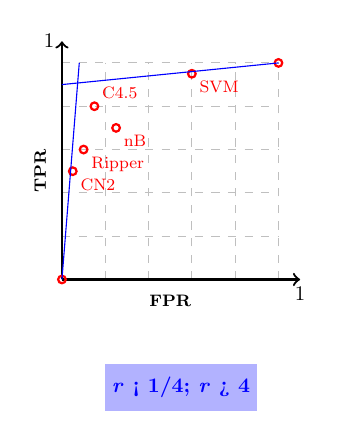
\begin{tikzpicture}[
		scale=2.75,
		every node/.style={scale=0.75}
	]

		\draw[step=0.2,lightgray,dashed] (0,0) grid (1,1);

		% axes
		\draw[->,thick] (0,0) -- (1.1,0) node[below]{1};
		\draw[->,thick] (0,0) -- (0,1.1) node[left]{1};

		\node at (0.5,-0.1) {\footnotesize \textbf{FPR}};
		\node[rotate=90] at (-0.1,0.5) {\footnotesize \textbf{TPR}};

		\draw[red,thick] (0,0) circle (0.5pt);
		\draw[red,thick] (0.05,0.5) circle (0.5pt) node[below right]{\footnotesize CN2};
		\draw[red,thick] (0.1,0.6) circle (0.5pt) node[below right]{\footnotesize Ripper};
		\draw[red,thick] (0.25,0.7) circle (0.5pt) node[below right]{\footnotesize nB};
		\draw[red,thick] (0.15,0.8) circle (0.5pt) node[above right]{\footnotesize C4.5};
		\draw[red,thick] (0.6,0.95) circle (0.5pt) node[below right]{\footnotesize SVM};
		\draw[red,thick] (1,1) circle (0.5pt);

		\draw[blue] (0,0.9) -- (1,1);
		\draw[blue] (0,0) -- (0.08,1);

		\node[blue,fill=blue!30,minimum height=8mm] at (0.55,-0.5) {\textbf{\textit{r} < 1/4; \textit{r} > 4}};
		
	\end{tikzpicture}
\end{figure}